\documentclass[12pt]{article}
\usepackage{graphicx} % Required for inserting images
\usepackage[letter,margin=1in]{geometry} % Adjust margins if needed
\usepackage[utf8]{inputenc}
\usepackage{hyperref}
\usepackage{url}
\usepackage{wrapfig}
\usepackage[
backend=biber,
style=nature,
]{biblatex}
\addbibresource{references.bib}

\begin{document}

\begin{center}
    \Large{\textbf{Grant Proposal: A Geospatial and Temporal Analysis of Lead Pollution From Piston Aircrafts Near Kelowna International Airport Using ICP-MS with ADS-B Data}}\\
    \vspace{1cm}
    \large{Wenqi Guo}\\
    \vspace{0.5cm}
    \textit{Project Duration: 2 months}\\
    \vspace{0.5cm}
    \textit{Funding Agency: UBC and Interior Health}\\
    \vspace{0.5cm}
    \textbf{Amount Required: \$1000}\\
    \vspace{1cm}
    \vspace{1cm}
    \today
\end{center}
\newpage

\section{Introduction and Background}
Lead has been known as a type of toxin and there is no known safe amount of lead: even a small amount of lead could lead to health issues, such as decreased IQ in children, high blood pressure, cardiovascular problems, and kidney damage. \cite{world_health_organization_lead_2023} Although leaded gasoline has been banned for on-road vehicles in the world, it is still used in many piston-engine powered small general aviation aircraft as 100LL (100 Low Lead), which contain tetraethyllead (TEL) and has a lead concentration of about 0.56g/L. 
\cite{noauthor_safety_2021} Although a past study shows the soil lead levels around Oklahoma airports are not higher than the level of concern, it did suggest long-term monitoring for soil lead levels. \cite{mccumber_geospatial_2017} More importantly, many other previous studies have shown that children near general aviation airports have elevated blood lead levels (BLL). \cite{miranda_geospatial_2011} \cite{zahran_leaded_2023} \cite{mills_lead_2022} \cite{zahran_effect_2017} Additionally, the United States Environmental Protection Agency has very recently issued a determination that lead-emission from position engine aircraft cause or contribute to air pollution, giving reasonable anticipation that it may endanger public health and welfare. \cite{us_epa_epa_2023}
% duzihlkouke rewrites

 However, it is not feasible to do blood or soil lead levels around every general aviation airport. 
 %THus/.. gangcaixiangsm wangjil   hexiamian UBCO youguankunduzkunyunzuibekuenx
 Another media report collected the Automatic Dependent Surveillance-Broadcast (ADS-B) data, which provides the tracking data of an aircraft's real-time information like location and altitude, and used the flight path and altitude to estimate lead exposure levels for the surrounding area. They mapped the flight frequency with altitudes lower than 10,000 feet. \cite{noauthor_you_2022} However, this is a semi-quantitative analysis: it might be reasonably accurate in estimating relative lead contamination for different areas, but it cannot give a numeric result of the amount of lead exposure and thus it cannot estimate the actual risk from lead exposure. 

Kelowna International Airport (CYLW) serves both commercial and general aviation airplanes. Although its location is remote from Kelowna downtown, it is not distanced from some residential neighborhoods such as Glenmore Highland and Rutland (about 5km and 4km to the end of CYLW runway, respectively). Given Kelowna's growing population and potential growth in residential areas, the close proximity of the airport is a valid public health concern. Additionally, the end of its runway is only about 1km from the University of British Columbia Okanagan Campus (UBCO), which is a growing educational and research institution with many students and staff, and there are about 2000 students who live on campus\footnote{\url{https://ok.ubc.ca/about/facts-and-figures/}}. This also raised concerns about possible lead contamination around the campus.

Another student project from UBCO analyzed the soil sample around the airport and found that the highest soil lead level is $11.55\pm 1.38$ mg/Kg, in Lake Country. \cite{citation_error:not_found} Values between 10-50 ppm do not have detrimental health effects. \cite{noauthor_lead_nodate} Although their study does consider the flight directions (flights usually take off on the south side and land on the north side), their geospatial resolution was low and did not combine with flight path data to analyze the effects of the flight path on soil lead level. Additionally, they did not consider the effects of wind direction on lead distribution: although flights are taking off southbound, they usually take off against the wind, meaning the wind is blowing toward the north side and could carry the lead particles to the north side of the airport. \cite{citation_error:not_found} Additionally, a soil sample is less time-sensitive when responding to aviation activities and might not be able to attribute the cause of lead in soil. 


% detial
In this study, we will collect the topsoil samples and air samples around the airport and analyze their lead level using ICP-MS. We will also collect the ADS-B data from the aircraft near CYLW from ADSB Exchange\cite{adsbexchange}. We will then analyze the geospatial and temporal correlation between the ADS-B data and lead level and determine if the air lead level is higher under the flight paths or when flight activities are more frequent. 
% can we also do airborn bisai biasiazuishbashouzhikunyunex
\section{Statement of Purpose}

Although leaded gasoline has been banned worldwide for on-road vehicles, it is still commonly used for small piston-engine powered general aviation (GA) aircraft. (The fuel commercial jets use is not led.) Previous study has shown that children near GA airports have elevated blood lead level.\cite{miranda_geospatial_2011} \cite{zahran_leaded_2023} \cite{mills_lead_2022} \cite{zahran_effect_2017} Kelowna International Airport is a busy airport that serves both GA and commercial aircraft. With the growing population in Kelowna and the UBCO campus, the lead emission from GA aircraft in this area is a public health concern. In this study, we aim to analyze the topsoil and air lead levels around the Kelowna International Airport using ICP-MS (an elemental analysis technique) to determine if there is a lead exposure concern for people living nearby and students and staff of UBCO. We will also incorporate it with the ADS-B data near the airport, which will provide the location and altitude information of the aircraft. This allows us to find the geospatial and temporal relations between the aircraft's activities and topsoil and air lead levels. The correlation could help us better understand how aviation activities affect soil lead levels and can help us build a model to predict soil lead levels using ADS-B data, providing an affordable alternative method for estimating soil lead levels compared to chemical analysis.
\section{Methods}
\subsection{Data Collection}
There are many ASD-B data providers on the market. In this study, we used the Application Programming Interface (API) from ADSBExchange \cite{adsbexchange} to capture the location information. We will capture the ADS-B data in 8 one-week time spans. The data capturing starts at 7 am on the first day of the week and ends at 10 pm on the last day of the week. During the capture, we request the API such that all the aircraft are within 50 nautical miles (about 92.6km) and we will log the data every 2 seconds. The data we are interested in are altitude, location (latitude and longitude), ICAO type designator (used to determine the engine type), vertical speed, and ground speed (used to predict the engine power and thus estimate the fuel consumption). At the same time, wind direction data around CYLW is also captured at the rate of once per minute. 

After capturing the data, we filter out flights with altitudes higher than 5000 feet, and then we look up the engine type of the aircraft using the ICAO type designator from ADSBExchange in the Aircraft Characteristics database \cite{faa}. For flight types that are not in the database, we manually look up their engine and labeled them. We use geopandas and Open Street Map \cite{OpenStreetMap} to overlay the flight paths onto a map. \footnote{The code to process the data could be found in \url{https://github.com/weathon/chem434/}}(A sample map was shown in \textbf{Figure} \ref{fig:map})

% something missing
\setlength\intextsep{0pt}
\begin{wrapfigure}{r}[1cm]{0.4\textwidth}
  \begin{center}
    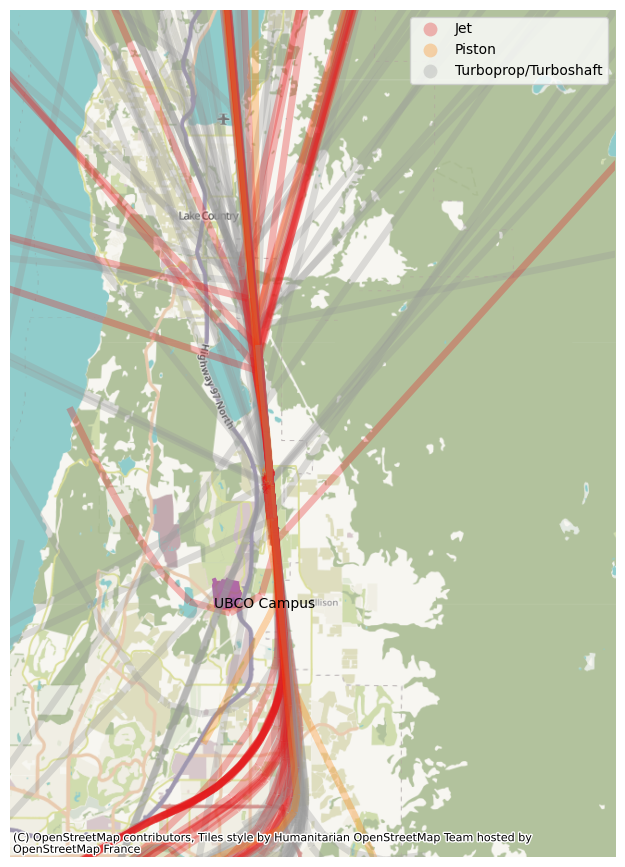
\includegraphics[width=0.4\textwidth]{download.png} \\
  \caption{Sample Map of Air Trafic Captured around CYLW on Nov 15, 2023}
      \label{fig:map}
  \end{center}
\end{wrapfigure}
This data will provide general information about the air traffic. However, not all aircraft broadcast their ADS information, especially small aircraft. At the same time, not all piston engines use 100LL. They could use unleaded gas or jet fuel. Thus, there might be some error between information from ADS-B and real leaded-gas-powered aircraft traffic. 



% not all broacattst saw many times
% not all uses avgas but most
% sample image


\subsection{Sample Collection And Analysis}
Since usually the airways are fixed and the flight paths would not deviate far from time, we will decide the sampling locations based on the flight path collected in the first week. We will collect the soil sample at locations at the busiest flight paths near the UBCO campus and 3 locations upwind and downwind of the location. At each location, we will collect 3 topsoil samples.  
\subsection{Data Analysis}
\section{Schedule}
\begin{center}
\begin{tabular}{|c|c|c|}
 \hline
 \textbf{Step} & \textbf{Begin Date} & \textbf{End Date} \\
 \hline \hline
Code for collection of ADS-B data & Nov 28, 2023 & Dec 1, 2023 \\
\hline
First Week ADS-B data collection & Dec 1, 2023 & Dec 7, 2023 \\
\hline
First Dirt Sample Collection & Dec 7 2023 & Dec 7, 2023 \\
\hline
First Air Sample Collection & Dec 7 2023 & Dec 7, 2023 \\
\hline
First batch of samples lab work & Dec 7, 2023 & Dec 8, 2023 \\ 
\hline
Second Week ADS-B data collection & Dec 8, 2023 & Dec 14, 2023 \\
\hline
Second Dirt Sample Collection & Dec 14 2023 & Dec 14, 2023 \\
\hline
Second Air Sample Collection & Dec 14 2023 & Dec 14, 2023 \\
\hline
First batch of samples lab work & Dec 14, 2023 & Dec 15, 2023 \\ 
\hline
Repeat for 3rd and 4th week & Dec 15, 2023 & Dec 29, 2023\\
\hline
All data processing and finishing the project& Jan 1, 2024 & Jan 29, 2024\\
\hline
\end{tabular}
\end{center}
\section{Conclusions}
\section{Budget and Justification}
\subsection{API Cost}\\

\newpage
\printbibliography
\end{document}
